
Project detail consists of two main sections divided into separate cards: project information and a list of processes (Figure~\ref{fig:project_detail}).

\begin{figure}[h!]
  \centering
  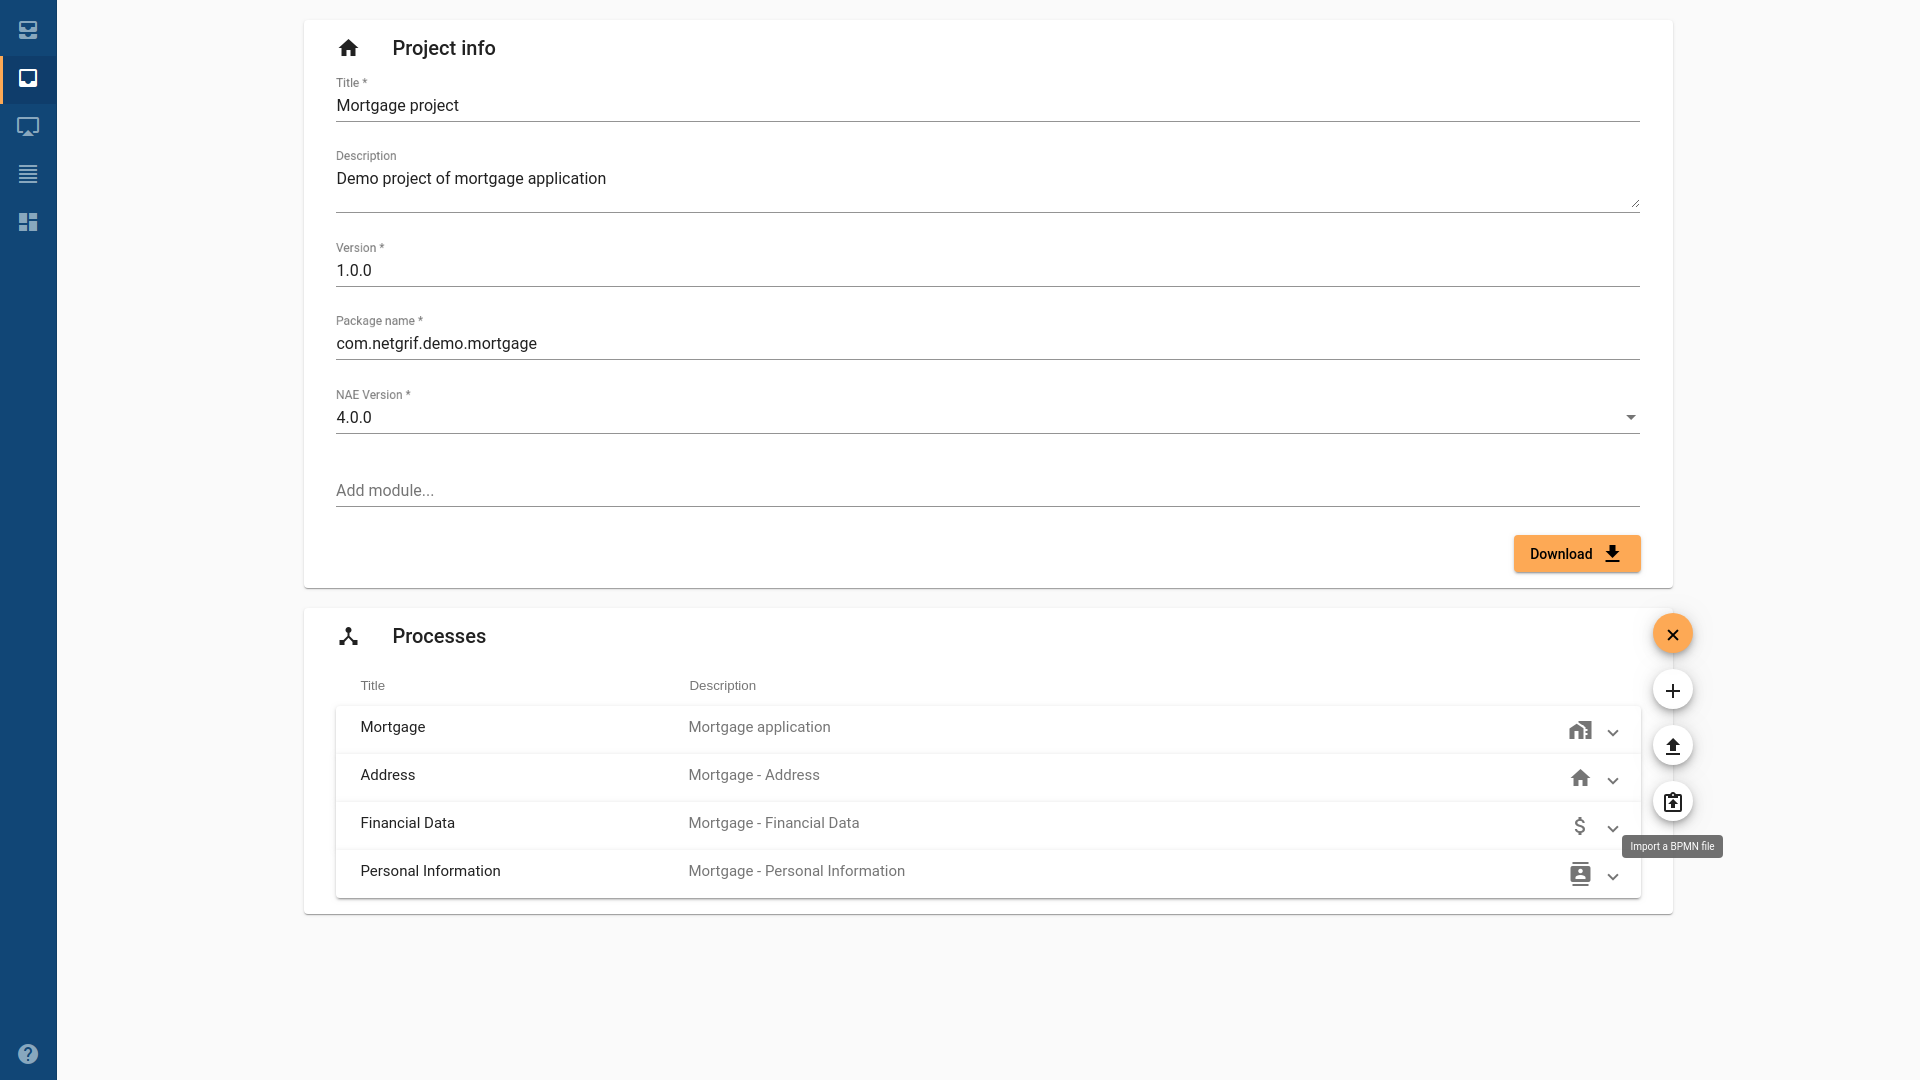
\includegraphics[width=0.9\textwidth]{images/project_view.png}
  \caption{Project detail}
  \label{fig:project_detail}
\end{figure}

\subsection{Project Info}\label{subsec:project-info}

Project info card shows all project metadata in an editable form:
\begin{itemize}
  \item title,
  \item description,
  \item version,
  \item package name - the name of the base Java package,
  \item NAE version - version of \engine~that will be used to run this project,
  \item modules.
\end{itemize}
Changes to any field are automatically saved.

At the bottom of the card, there is a \texttt{Download} button that will compress the project configuration file and all processes into a single zip file.
Projects are currently not saved to any server and leaving the \builder~will result in the loss of all projects.

\subsection{Processes}\label{subsec:processes}

This card shows a list of all processes in the current project.
Processes are sorted in the order as they were created.
To change the sorting simply click on the \texttt{Title} of \texttt{Description} header.
After each click the sorting cycles through different orders as follows: ascending order, descending order and no order.

Each process is initially displayed as a single list item showing its title, description and icon.
After clicking on the process the item expands and additional data are shown in an editable form:
\begin{itemize}
  \item title,
  \item case title - default title of a new case,
  \item description,
  \item version,
  \item initials,
  \item icon - any Material Design icon can be used, a list of all icons is available at \url{https://material.io/resources/icons/},
  \item identifier - unique string identifying the process.
\end{itemize}
Changes to any field are automatically saved.
At the bottom of the process detail there are two buttons \texttt{Delete} and \texttt{Open}.
Clicking on the Delete button deletes the process.
Clicking on the Open button will redirect you to the \hyperref[sec:modeler]{Modeler view} where the process is displayed.

A new process can be added to the project by clicking the fast action button on the right border of the card and selecting one of the following options:
\begin{itemize}
  \item new process - creates an empty process model,
  \item import an existing process - opens a file dialog where you can choose an XML file of a Petriflow model,
  \item import a BPMN file - opens a file dialog where you can choose a BPMN file which will be transformed and imported into the project.
\end{itemize}
After that a new item is added to the list of processes.
